\documentclass[plain]{article}
\usepackage{lipsum}
\setlength{\oddsidemargin}{0.25 in}
\setlength{\evensidemargin}{-0.25 in}
\setlength{\topmargin}{-0.6 in}
\setlength{\headsep}{0.75 in}
\setlength{\parindent}{0 in}
\textwidth 6.1in
\textheight 9in
\parskip 1ex
\usepackage[framemethod=TikZ]{mdframed}
%
% ADD PACKAGES here:

 \newcommand{\argmax}{\operatornamewithlimits{argmax}}
 \usepackage[colorinlistoftodos]{todonotes}
\newcommand{\Ex}{\mathbb{E}}
\usepackage{psfrag}
\usepackage{amsmath,amsfonts,graphicx}
\usepackage{amssymb}
\usepackage{tikz}
\usepackage{mathtools}
\usepackage{bbm}
\usepackage{hyperref}
\usepackage{bm}
\usepackage{float}
\usepackage{flexisym}
\usepackage[short]{optidef}
\usepackage{caption}
\usepackage{subcaption}
\usetikzlibrary{shapes,arrows,calc}
\newtheorem{thm}{Theorem}
\newtheorem{example}{Example}
\newtheorem{defin}{Definition}
\newtheorem{defn}{Definition}
\newtheorem{rem}{Remark}
\usepackage{framed}
\newcommand{\Pd}{\mathbb{P}}
\newtheorem{algorithm}{Algorithm}
\newtheorem{fact}{Fact}
\usepackage{natbib}
 \newcounter{lecnum}

\newcommand{\EE}{ \mathsf{E} }
\newcommand{\Var}{ \mbox{Var} }
\newcommand{\Cov}{ \mbox{Cov} }
\newcommand{\1}{\mathbbm{1}}
\newcommand{\Prob}{ \mathsf{P} }
\newcommand{\disfrac}[2]{ {\displaystyle \frac{#1}{#2}} }
\newcommand{\texfrac}[2]{ {\textstyle \frac{#1}{#2}} }
\newcommand{\dissum}[2]{ {\displaystyle \sum_{#1}^{#2}} }
\newcommand{\OR}{ \mbox{~or~} }
\newcommand{\cond}[1]{ \left|\,#1\right. }
\newcommand{\ith}[1]{ #1^{\mbox{\tiny th}} }
\newcommand{\matgen}[1]{ \left[ \begin{array}#1 \end{array} \right] }

\newcommand{\RR}{ {\bf R} }
\newcommand{\NN}{ {\bf N} }
\newcommand{\II}{ {\bf I} }
\newcommand{\ee}{ {\bf e} }
\newcommand{\LL}{ {\bf L} }
\newcommand{\PP}{ {\bf P} }
\newcommand{\calF}{ {\cal F} }
\newcommand{\One}{ \mbox{\sffamily 1} }
\newcommand{\ZZ}{ {\bf Z} }
\newcommand\E{\mathbb{E}}

\newcommand{\R}{{\sf R\hspace*{-0.9ex}%
\rule{0.15ex}{1.5ex}\hspace*{0.9ex}}}
\newcommand{\N}{{\sf N\hspace*{-1.0ex}%
\rule{0.15ex}{1.3ex}\hspace*{1.0ex}}}
\newcommand{\Q}{{\sf Q\hspace*{-1.1ex}%
\rule{0.15ex}{1.5ex}\hspace*{1.1ex}}}
\newcommand{\C}{{\sf C\hspace*{-0.9ex}%
\rule{0.15ex}{1.3ex}\hspace*{0.9ex}}}

\newcommand{\ds}{ \displaystyle }
\bibliographystyle{plain}
%
% The following macro is used to generate the header.
%
\newcommand{\lecture}[4]{
   \pagestyle{myheadings}
   \thispagestyle{plain}
   \newpage
   \noindent
   \begin{center}
   \framebox{
      \vbox{\vspace{2mm}
    \hbox to 6.28in { {\bf Subject}
	\hfill \today} 
       \vspace{4mm}
       \hbox to 6.28in { {\Large \hfill #1  \hfill} }
       \vspace{2mm}
       \hbox to 6.28in { {\hfill \it } }
      \vspace{2mm}
       \hbox to 6.28in { {\hfill \it Author: #2} }
      \vspace{2mm}}
   }
   \end{center}
   \markboth{#1 (#2)}{#1}
   \vspace*{4mm}
}
\usepackage{hyperref}
\usepackage[T1]{fontenc}
\usepackage[utf8]{inputenc}
\usepackage{textcomp} % provide euro and other symbols

\let\b\mathbf

%Use this command for a figure; it puts a figure in wherever you want it.
%usage: \fig{NUMBER}{SPACE-IN-INCHES}{CAPTION}
\newcommand{\fig}[3]{
			\vspace{#2}
			\begin{center}
			Figure \thelecnum.#1:~#3
			\end{center}
	}

\newtheorem{theorem}{Theorem}[lecnum]
\newtheorem{lemma}[theorem]{Lemma}
\newtheorem{proposition}[theorem]{Proposition}
\newtheorem{claim}[theorem]{Claim}
\newtheorem{corollary}[theorem]{Corollary}
\newtheorem{definition}[theorem]{Definition}
\newenvironment{proof}{{\bf Proof:}}{\hfill\rule{2mm}{2mm}}

\begin{document}
\lecture{Notes}{Bryan Tantisujjatham}{1}

\makeatother
\setlength{\emergencystretch}{3em} % prevent overfull lines
\providecommand{\tightlist}{%
  \setlength{\itemsep}{0pt}\setlength{\parskip}{0pt}}
\author{Bryan Tantisujjatham}
\date{\today}

\todototoc
\listoftodos
\section{Carbon Free Emissions Plan}
\section{Nationwide Trends}

\section{Current Statistics}


\section{Quantitative Data Analysis}
Population of NYS 19.45 million as of 2019 \cite{noauthor_us_nodate}\\
Population of NYC 8.149 million as of 2019 (cite census)\\

\begin{align*}
	\text{LCOE} = \frac{\text{total annualized cost}}{\text{total annual energy output}}	
.\end{align*}

LCOE should be around 63/MWh for hydro, 32/MWh for land wind, 96/MWh for offshore-wind, 41/MWh for utility solar, 73/MWh for community distributed solar, 297/MWh based on 2019 NYISO numbers
\section{Electricity Demand Forecast}
\begin{figure}[H]
	\centering
	\includegraphics[width=0.5\textwidth]{load_zones.png}
	\caption{}
	\label{fig:}
\end{figure}
\section{Need}
Amount of dispatchable need increases to 32,000 MW in 2040 under CLCPA assumptions

Load: Climiate change and electrification results in increase in summer load\\
Electrification will transition NY from summer peaking to winter peaking
Winter peak load under CLCPA will dobule
Projected by 2040: 47KMW, winter peak over 57kMW
\\
Need for dispatchable resources that perform on a multi-day period to maintain bulk power system reliability. No commercially available systems.\\

Increased need for transmission systems that accomodate more quantities of dispatchable energy.\\
We require the dispatchable resources to be fossil fuel free, and accomodate high ramping requirements as seen for sun and wind resources.\\
Reliability metrics: \textbf{transmission security} and \textbf{resource adequacy}.\\
Transmission security margins: \textbf{how robust the model is to distributional shift} \\
Loss of load expectation (days per year) (LOLE)
Loss of load hours (hours per year) (LOLH)\\
Expected unserved energy (megawatt-hours per year)\\

\subsection{Transmission}

\subsection{Inverter based resources}
wehoiw
\section{Accounting for uncertainty in project planning}

Analysis of load, generation, demand, transmission

\section{NN Architecture}
Hyperparameter Tuning, 4 Linear layers with Dropout = 0.3 and ReLU activation \\
Batch size is 64, hidden dim is 64
\todo{include dataset description}
\subsection{Related Methods}
Fuzzy logic, genetic algorithms, regression
\subsection{Methods}
\subsection{ARIMA}
\subsection{Support Vector Regression}
\subsection{LSTM}
\section{New sources of generation}
\subsection{Wind}

\subsubsection{Land}

\subsubsection{Offshore}
New offshore wind projects in pipeline:
\begin{tightlist}
	\item \textbf{Empire Wind 1}: 816 MW, solicited 2018 \cite{noauthor_new_nodate-1}
	\item \textbf{Empire Wind 2}: 1260 MW, solicited 2020 \cite{noauthor_new_nodate-1}
	\item \textbf{Sunrise Wind}: 880 MW, solicited 2018 \cite{noauthor_new_nodate-1}
	\item \textbf{Beacon Wind}: 1230 MW, solicited 2020 \cite{noauthor_new_nodate-1}
\end{tightlist}

5 total projects totaling greater than 4300 MW, leading offshore generation pipeline in the nation

Official target goal for offshore wind generation is 9000 MW by 2035. \cite{noauthor_us_nodate-1}

Substation Locations: Astoria Substation, Gowanus Substation, Barrett Substation, Holbrook Substation, East Hampton Substation\\
Proposed Port Facilities: South Brooklyn Marine Terminal, Holbrook Substation, East Hampton Substation. \cite{noauthor_new_nodate-1}

All projects are currently in the data collection phase. \cite{noauthor_new_nodate-1}

NYSERDA offers contracts to purchase offshore renewable energy certificates (OREC) from offshore wind developers. NYSERDA sells these to load serving entities (LSEs) like utilities, which are required by law to purchase renewable energy credits. \cite{NYSERDA_new_nodate-1}

\subsubsection{Technology \& Implementation}
Advances in:
\begin{enumerate}
	\item Materials
	\item Engineering of turbine foudnations
	\item Turbine blade design
\end{enumerate}

With respect to foundations: \cite{mitchell_review_2022}
\begin{enumerate}
	\item Monopiles - for depths up to 25m. Freestanding; cheap, easy to install and inexpensive to manufacture and transport. Used in 95\& of installations worldwide.
	\item Gravity - also for up to 25m, but used for les cohesive seabed compositions
	\item Suction bucket - Can also be cost effective, but oly for appropriate choice of seabed composition
	\item Deepwater - 
	\item Tripod - 30m - 60m water depth
	\item Jacket - > 50m water depth. Expensive and complex to install and manufacture; however, mature
\end{enumerate}
\subsubsection{Geography of the Long-Island Area}

\subsection{Solar}
Official target: 10GW distributed solar by 2030 (cite NYSERDA)\\
Government sponsored incentives via tax credits, NYSun

\subsection{Geothermal}
\section{Maintenance of mature technologies and infrastructure}
\subsection{Nuclear}



\section{Policy Changes}
NYSERDA energy credits:
	\begin{enumerate}
		\item Tier 1 (new renewables)
		\item Tier 2 (maintenance resources)
		\item Tier 2 (competitive program)
		\item Tier 4 (NYC renewable energy)
	\end{enumerate}
\subsection{Pricing Changes}
\subsection{Economic viability}
Need Fair distribution of costs between ISOs and RTOs. \cite{mitchell_review_2022}\\
Renewable Portfolio Standards\\
Aggressive federal support amenable to policy decision to focus on offshore wind -- allows ISOs to reach LCOE  levels for offshore installation costs similar to those seen in the UK, given the tax subsidies \cite{mitchell_review_2022}\\

\section{Viability (outside of financial)}
\subsection{Resource constraints}
\subsection{Trend constraints}
\subsection{Location constraints}
\section{Background}
The last two decades have brought marked improvements in energy efficient systems and infrastructure on a global scale. The penetration profile of electricity generation sources has seen a nationwide trend towards renewable and "clean" energy source -- offshore wind, nuclear, biofuels, and geothermal -- and a complementary shift away from traditional fossil fuels. 

The NYISO region is uniquely characterized by the speed at which it has adopted -- and integrated -- new technologies and developed infrastructure. It remains the only coal free region in the US, and leads the nation in installed capacity of several renewable sources -- most notably offshore wind \cite{noauthor_new_nodate-1} \todo{check citation}. With five offshore wind projects in active development, New York is touted as the nation's "hub" for offshore wind, projecting to deliver approximately 4300 MW from these facilities alone, with goals to extend that to 9000 MW by 2040 \todo{citation}. Quite remarkably, New York consumes less total energy per capita than all but two states, and \todo{a little more here?}.

While the NYISO has released a comprehensive plan towards 70\% renewable energy by 2030, and 100\% carbon-free electricity by 2040, 
there are several areas which remain unexploited. Our work aims to assess these areas of untapped potential and improvements in policy that can be leveraged to accelerate progress towards a more ambitious goal -- how the NYISO region can be \textit{fossil fuel free} by 2030. In particular, we \todo{cite main suggestions} We also provide a robust, quantitative analysis of projected energy demand and projected generation requirements needed to sustain this trend towards 100\% carbon-free electricity in the next eight years.

\subsection{Statewide Energy Profile}
New York has consistently met nearly 90\% of energy requirements through nuclear, hydropower and natural gas alone. In 2020, New York accounted for nearly 11\% of U.S. hydroelectricity generation, and was the third largest producer of hydroelectricity in the nation \todo{citation}.Renewable resources were responsible for nearly 60\% of electricity generation alone that same year. Figure 1 shows the profile of electricity generation distributed across different sources as of March 2022. The 

\missingfigure{}
In recent years, the distribution has undergone a marked shift away from nuclear. Indian Point, responsible for nearly 25\% of the state's electricity generation \cite{mcgeehan_indian_2021}, of carbon free electricity, permanently shut down by April 2021. With a capacity factor of nearly 90\%, facility delivered reliable base load electricity across the state, and its closure produced a void of approximately 2000MW of nuclear generating capacity. Since then, the share of the state's power from gas-fired generators has increased, jumping nearly 6\% since the closure of its last unit (Indian Point Unit 3) in 2021. \todo{double check statistics}.
\\
With regards to the cost of electricity, average retail price is the 8th highest in the nation as of 2022, fluctuating between 20 and 22 cents per kWh.

\subsubsection{Imports}
For zones A-E receive hydro imports from the Quebec region, and the Tier 4 NYC project is responsible for serving downstate (zones F-K) load.
\subsection{Current Plans}
According to the Zero Emissions Electric grid in NY by 2040 study, New York is on track to meeting 70\% of electricity generation from renewables by 2030. Interestingly, zones A-E, serving all of upstate new york, are on track to having 100\% of emissions completely carbon free. \todo{cite NYSERDA}. The key bottleneck is in Zones F-K, which serve downstate and is projected to meet 80\% of its load with zero emissions resources by 2030. \todo{cite NYSERDA}.


\begin{figure}[H]
	\centering
	\includegraphics[width=0.8\textwidth]{}
	\caption{}
	\label{fig:}
\end{figure}

\section{Transmission}


\subsection{Technology}

\subsection{Policy}
\subsubsection{NYSUN}
\begin{enumerate}
	\item NYSun PV
\end{enumerate}
\subsubsection{Tax Credits and Subsidies}
\begin{enumerate}
	\item Solar Energy System Equipment Credits
	\item OREC for offshore wind solicitatoins
	\item 
\end{enumerate}

\subsection{Infrastructure}

\subsection{Control}
Recent innovations in in statistical modeling, in particular data-driven optimization and machine learning, have severely overhauled the standard procedures and conventional lines of thinking for management of electricity on the grid. Interest in smart-buildings and online optimization techniques for realtime energy usage has exploded \cite{yu_review_2021}, \cite{khan_modeling_2022}, \cite{sembroiz_planning_2019}, especially with the advent of reinforcement learning and robust model predictive control \cite{chen_efficient_2020}, \cite{yang_adaptive_2019}. \todo{more RL citations}. Closely related are the capacity to accurately monitor systems and detect real-time faults. According to Bloomberg New Energy finance, U.S. utilities invested approximately  \$3.4 billion in smart grid technologies at the distribution level, and since 2008, \$31.6 billion on the same, a much higher rate than initial forecasts. Smart grids promise to introduce several benefits on the control level, including increased efficiency and monitoring in transmission, voltage optimization in distribution system technologies, advanced metering infrastructure, and easier accessibility to energy usage data on the individual (consumer) level. \cite{cite energy.gov}. 


According to a 2010 NIST report, the challenges to adoption of Smart Grid technology can be roughly categorized into three needs that must be fulfilled: 1) smart infrastructure, 2) smart management systems, and 3) smart protection \cite{moreno_escobar_comprehensive_2021-1}. Furthermore, investment and development in each of these areas must be considered carefully on the transmission and distribution level. We argue that the current state of optimization and control technologies, as well as the unique geographical load profile of the New York region, is amenable to seeing this vision to its fruition, outlined in the next four sections.

\subsection{Smart infrastructure}
Although NYSERDA has invested in approximately \$65 million in awards to support the development of a statewide smart grid, we claim this investment must be increased, particularly in supporting incremental and experimental changes on the distribution level. The primary focus should not be on construction of new buildings that conveniently support this technology, but accelerated "retrofitting" of existing buildings with smart meters, monitoring tools and residential interfaces for local clusters.
Funds have been mostly divested in feasibility studies and research projects, which advance the technical side, but one of the main barriers to adoption is the lack of regulatory framework and low public awareness and engagement. Previous barriers to entry, such as the lack of open standards, cybersecurity and data privacy concerns, lack of infrastructure, and shortage of experts with relevant technical skills, have been significantly addressed within the last 5 years, due to the explosion in interest in machine learning and distributed systems and resultant efforts to enact regulations on data privacy and AI fairness \todo{cite source}.

\subsection{Smart management systems}


\subsection{Smart protection}
Increasing standardization of mass data collection systems in the private and public sector have led to rising concerns of privacy and equity with respect to smart systems. 

\subsubsection{Microgrids}
Several research institutes, including NREL, Berkeley Lab, Sandia National Laboratory, and the EPRI, have developed robust microgrid simulation software capable of multiobjective optimization and a systems engineering approach to modeling complex electrical and thermal energy demand requirements, both with respect to dynamics and economic feasibility. \todo{cite microgrid resources.org}. Furthermore, the emergence of DC technologies and proliferation of IoT devices will help smart grid systems scale naturally with existing infrastructure \todo{\cite microgrid resources.org}.

\subsubsection{Other things to possibly include}
\begin{enumerate}
	\item statistics on how 
\end{enumerate}
\section{Quantitative Analysis}
We first sought to characterize the energy load, demand, transmission and generation profiles on annual and monthly timescales, as well as obtain projected estimates until 2030. Figures of total energy consumption, generation, and consumption for electricity generation are shown in the figures below.

\subsubsection{ARIMA}
ARIMA, or AutoRegressive Integrated Moving Average, is a commonly used method for time series analysis. Due to the diurnal nature of electricity demand, we implemented a seasonal ARIMA model. Formally, ARIMA is described by the equations
\begin{align}
&y_{t}^{*}=\Delta^{d} y_{t} \\
&y_{t}^{*}=\mu+\underbrace{\sum_{i=1}^{p} \phi_{i} y_{t-i}^{*}}_{\mathrm{AR}}+\underbrace{\sum_{i=1}^{q} \theta_{i} \epsilon_{t-i}+\epsilon_{t}}_{\mathrm{MA}}
\end{align}
where $\mu$ denotes the mean.

A seasonal arima model is of the form 
\begin{align}
	\text{ARIMA}(p,q) \times (P,Q)_s
.\end{align}


where 

\subsubsection{LSTM}
We additionally generated yearly predictions using a Long Short Term Memory RNN model, given that neural function approximation is more expressive and tends to lead to less generalization error than statistical regression techniques. Formally, an LSTM unit is described by the equations

\begin{align}
f_{t} &=\sigma_{g}\left(W_{f} x_{t}+U_{f} c_{t-1}+b_{f}\right) \\
i_{t} &=\sigma_{g}\left(W_{i} x_{t}+U_{i} c_{t-1}+b_{i}\right) \\
o_{t} &=\sigma_{g}\left(W_{o} x_{t}+U_{o} c_{t-1}+b_{o}\right) \\
c_{t} &=f_{t} \circ c_{t-1}+i_{t} \circ \sigma_{c}\left(W_{c} x_{t}+b_{c}\right) \\
h_{t} &=o_{t} \circ \sigma_{h}\left(c_{t}\right)
\end{align}
where $i$ denotes the input, $h$ denotes the output of the hidden layer, $o$ denotes the output of the output layer, and c and f are \todo{complete}.
\subsubsection{Support Vector Regression}

Primal Formulation:
\begin{figure}[H]
	\centering
	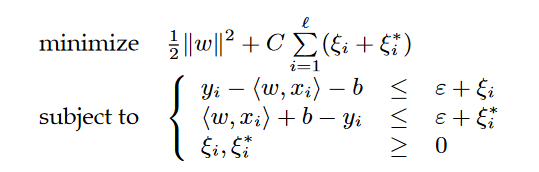
\includegraphics[width=0.5\textwidth]{svm_primal.PNG}
	\caption{}
	\label{fig:}
\end{figure}

Dual Formulation:
\begin{figure}[H]
	\centering
	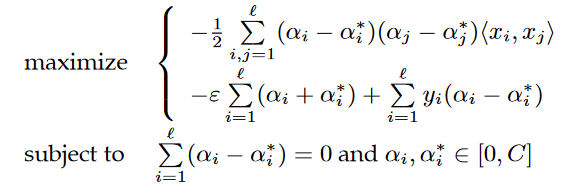
\includegraphics[width=0.5\textwidth]{svm_dual.PNG}
	\caption{}
	\label{fig:}

\end{figure}

\subsubsection{Comparisons to Existing Models}


\section{Limitations}
\begin{enumerate}
	\item Lack of quantitative analysis on the impact of increased investment to smart grids - mention that doing an SSI M and a reachability matrix is out of the scope of this class
	\item 
\end{enumerate}
\bibliography{cite}
\end{document}
